\documentclass[conference]{IEEEtran}
\IEEEoverridecommandlockouts
% The preceding line is only needed to identify funding in the first footnote. If that is unneeded, please comment it out.
\usepackage{cite}
\usepackage{amsmath,amssymb,amsfonts}
\usepackage{algorithmic}
\usepackage{graphicx}
\usepackage{textcomp}
\usepackage{xcolor}
\usepackage{microtype} % Helps with justification and overflow
% \usepackage{url} % Replaced by hyperref
\usepackage[colorlinks=true, urlcolor=cyan, linkcolor=black, citecolor=black, filecolor=black]{hyperref} % Added for styled links

\def\BibTeX{{\rm B\kern-.05em{\sc i\kern-.025em b}\kern-.08em
    T\kern-.1667em\lower.7ex\hbox{E}\kern-.125emX}}

% Optional: Add hyphenation for specific problematic words if known
% \hyphenation{kata-sulit-dihyphenasi}

\begin{document}

\title{Implementasi Regresi Polinomial untuk Analisis Data Eksperimental}

\author{\IEEEauthorblockN{Fathan Yazid Satriani}
\IEEEauthorblockA{\textit{Departemen Teknik Elektro} \\
\textit{Universitas Indonesia}\\
Depok, Indonesia \\
NPM: 2306250560}
}

\maketitle

\begin{abstract}
Regresi polinomial adalah metode statistik yang digunakan untuk memodelkan hubungan antara variabel independen dan variabel dependen sebagai polinomial derajat ke-n. Proyek ini mengimplementasikan algoritma regresi polinomial menggunakan bahasa C++ untuk menganalisis set data eksperimental. Program membaca data dari file, menghitung koefisien polinomial menggunakan metode normal equations yang diselesaikan dengan eliminasi Gauss, dan menyimpan koefisien tersebut. Selanjutnya, skrip Python digunakan untuk memvisualisasikan data asli dan kurva polinomial yang dihasilkan, memberikan representasi grafis dari kecocokan model. Studi kasus ini menunjukkan penerapan regresi polinomial dalam menemukan tren pada data yang mungkin tidak linear secara sederhana. Hasilnya menunjukkan bahwa metode ini efektif dalam mengaproksimasi fungsi yang mendasari data dengan tingkat akurasi yang bergantung pada derajat polinomial yang dipilih dan sifat data itu sendiri.
\end{abstract}

\begin{IEEEkeywords}
regresi polinomial, metode numerik, pencocokan kurva, C++, Python, analisis data
\end{IEEEkeywords}

\section{Pendahuluan}
Dalam analisis data, seringkali kita dihadapkan pada kebutuhan untuk memahami dan memodelkan hubungan antara berbagai variabel. Salah satu teknik fundamental dalam pemodelan statistik dan pembelajaran mesin adalah regresi. Ketika hubungan antara variabel independen (x) dan variabel dependen (y) tidak bersifat linear, regresi linear sederhana mungkin tidak cukup untuk menangkap pola yang mendasarinya. Regresi polinomial memperluas konsep regresi linear dengan memodelkan hubungan ini sebagai polinomial derajat ke-n.

Metode ini sangat berguna dalam berbagai bidang ilmu pengetahuan dan teknik, di mana data eksperimental seringkali menunjukkan tren non-linear. Contohnya termasuk pemodelan pertumbuhan populasi, analisis data sensor, prediksi kinerja material, dan banyak lagi. Dengan menyesuaikan derajat polinomial, kita dapat mencapai keseimbangan antara kecocokan model dengan data (goodness-of-fit) dan kompleksitas model untuk menghindari overfitting.

Proyek UAS ini berfokus pada implementasi metode regresi polinomial dari awal menggunakan bahasa pemrograman C++. Tujuannya adalah untuk mengembangkan program yang dapat menerima satu set titik data (x, y), menentukan koefisien dari polinomial yang paling sesuai dengan data tersebut untuk derajat yang ditentukan, dan kemudian memvisualisasikan hasilnya. Visualisasi akan dilakukan menggunakan Python dengan pustaka Matplotlib, yang akan menampilkan titik data asli bersama dengan kurva regresi polinomial yang dihitung.

Laporan ini akan menjelaskan secara rinci dasar-dasar teori regresi polinomial, metodologi implementasi dalam C++, data yang digunakan untuk pengujian, analisis hasil eksperimen termasuk plot yang dihasilkan, dan kesimpulan dari proyek ini.

\section{Studi Literatur}
Regresi polinomial adalah jenis analisis regresi di mana hubungan antara variabel independen $x$ dan variabel dependen $y$ dimodelkan sebagai polinomial derajat $n$ dalam $x$. Persamaan regresi polinomial dapat ditulis sebagai:
\begin{equation}
y = a_0 + a_1x + a_2x^2 + \dots + a_nx^n + \epsilon
\label{eq:poly_reg_func}
\end{equation}
di mana $a_0, a_1, \dots, a_n$ adalah koefisien regresi yang perlu diestimasi, dan $\epsilon$ adalah error acak atau residual. Tujuan dari regresi polinomial adalah untuk menemukan nilai koefisien-koefisien ini sehingga jumlah kuadrat residual (Sum of Squared Residuals, SSR) diminimalkan.

Metode yang umum digunakan untuk menemukan koefisien ini adalah metode kuadrat terkecil (least squares method). Untuk $m$ titik data $(x_i, y_i)$, kita ingin meminimalkan:
\begin{equation}
S = \sum_{i=1}^{m} (y_i - (a_0 + a_1x_i + a_2x_i^2 + \dots + a_nx_i^n))^2
\label{eq:sum_sq_residuals}
\end{equation}
Untuk meminimalkan $S$, kita mengambil turunan parsial dari $S$ terhadap setiap koefisien $a_j$ dan menyamakannya dengan nol. Hal ini menghasilkan sistem persamaan linear yang dikenal sebagai \textit{normal equations}. Untuk polinomial derajat $n$, sistem ini terdiri dari $n+1$ persamaan linear dalam bentuk umum:
\begin{align}
m a_0 + (\sum x_i) a_1 + \dots + (\sum x_i^n) a_n &= \sum y_i \nonumber \\
(\sum x_i) a_0 + (\sum x_i^2) a_1 + \dots + (\sum x_i^{n+1}) a_n &= \sum x_i y_i \label{eq:normal_equations_expanded} \\
\vdots \quad &= \quad \vdots \nonumber \\
(\sum x_i^n) a_0 + (\sum x_i^{n+1}) a_1 + \dots + (\sum x_i^{2n}) a_n &= \sum x_i^n y_i \nonumber
\end{align}
Sistem persamaan linear ini dapat ditulis secara lebih ringkas dalam bentuk matriks sebagai:
\begin{equation}
\mathbf{X}^T\mathbf{X}\mathbf{A} = \mathbf{X}^T\mathbf{Y}
\label{eq:normal_equations_matrix_form}
\end{equation}
di mana $\mathbf{X}$ adalah matriks desain, $\mathbf{A}$ adalah vektor koefisien, dan $\mathbf{Y}$ adalah vektor nilai dependen. Matriks $\mathbf{X}$ untuk $m$ data poin dan polinomial derajat $n$ adalah:
\begin{equation}
\mathbf{X} = \begin{bmatrix}
1 & x_1 & x_1^2 & \dots & x_1^n \\
1 & x_2 & x_2^2 & \dots & x_2^n \\
\vdots & \vdots & \vdots & \ddots & \vdots \\
1 & x_m & x_m^2 & \dots & x_m^n
\end{bmatrix}
\label{eq:design_matrix_X}
\end{equation}
Vektor koefisien $\mathbf{A}$ dan vektor nilai dependen $\mathbf{Y}$ adalah:
\begin{equation}
\mathbf{A} = \begin{bmatrix} a_0 \\ a_1 \\ \vdots \\ a_n \end{bmatrix}, \quad
\mathbf{Y} = \begin{bmatrix} y_1 \\ y_2 \\ \vdots \\ y_m \end{bmatrix}
\label{eq:vectors_A_Y}
\end{equation}
Sistem normal equations (Persamaan \ref{eq:normal_equations_matrix_form}) kemudian dapat diselesaikan untuk $\mathbf{A}$ menggunakan berbagai metode aljabar linear, seperti eliminasi Gauss atau dekomposisi LU \cite{b1}. Pemilihan derajat polinomial $n$ adalah aspek penting. Derajat yang terlalu rendah dapat menyebabkan underfitting (model terlalu sederhana), sedangkan derajat yang terlalu tinggi dapat menyebabkan overfitting (model terlalu kompleks dan menangkap noise dalam data) \cite{b2}.

\section{Penjelasan Data Yang Digunakan}
Untuk proyek ini, data yang digunakan adalah data sintetis yang dihasilkan untuk meniru tren polinomial dengan sedikit noise acak. Data ini disimpan dalam file teks bernama \texttt{data.txt} di dalam direktori \texttt{Program}. Setiap baris dalam file ini merepresentasikan satu titik data $(x, y)$, dengan nilai $x$ dan $y$ dipisahkan oleh spasi.

Contoh format data dalam \texttt{data.txt}:
\begin{verbatim}
0.0 1.1
0.5 1.8
1.0 2.7
1.5 4.5
2.0 5.8
2.5 8.0
3.0 10.1
3.5 13.5
4.0 17.3
4.5 21.0
5.0 25.5
5.5 30.0
6.0 36.2
\end{verbatim}
Data ini dipilih untuk memberikan serangkaian titik yang secara visual menunjukkan tren non-linear, sehingga cocok untuk dianalisis menggunakan regresi polinomial. Program C++ akan membaca data ini untuk melakukan perhitungan regresi. Skrip Python juga akan membaca file data yang sama untuk memplot titik-titik data asli bersama dengan kurva regresi yang dihasilkan.

Penggunaan data sintetis memungkinkan kita untuk memiliki kontrol atas karakteristik data dan mempermudah verifikasi kebenaran implementasi metode numerik. Dalam kasus nyata, data ini bisa berasal dari berbagai sumber eksperimental atau observasional.

\section{Penjelasan Metode Yang Digunakan}
Metode utama yang diimplementasikan dalam proyek ini adalah regresi polinomial menggunakan metode kuadrat terkecil untuk menentukan koefisien polinomial. Algoritma diimplementasikan dalam bahasa C++ dan langkah-langkah utamanya adalah sebagai berikut:

\begin{enumerate}
    \item \textbf{Pembacaan Data}: Program C++ pertama-tama membaca titik-titik data $(x_i, y_i)$ dari file \texttt{Program/data.txt}. Setiap titik data disimpan dalam sebuah struktur atau kelas yang sesuai.
    \item \textbf{Penentuan Derajat Polinomial}: Derajat polinomial $n$ yang akan dicocokkan ditentukan oleh pengguna (dalam kode, ini diatur sebagai variabel, misalnya `polynomialDegree = 2` untuk polinomial kuadratik).
    \item \textbf{Pembentukan Normal Equations}: Berdasarkan titik data yang dibaca dan derajat polinomial $n$, program membentuk sistem normal equations (Persamaan \ref{eq:normal_equations_matrix_form}).
    \begin{itemize}
        \item Matriks $\mathbf{X}^T\mathbf{X}$ adalah matriks $(n+1) \times (n+1)$ yang elemennya $(j, k)$ adalah $\sum_{i=1}^{m} x_i^{j+k}$, di mana $j, k$ berkisar dari $0$ hingga $n$.
        \item Vektor $\mathbf{X}^T\mathbf{Y}$ adalah vektor $(n+1) \times 1$ yang elemennya $j$ adalah $\sum_{i=1}^{m} y_i x_i^j$.
    \end{itemize}
    \item \textbf{Penyelesaian Sistem Persamaan Linear}: Sistem normal equations yang terbentuk kemudian diselesaikan untuk mendapatkan vektor koefisien $\mathbf{A} = [a_0, a_1, \dots, a_n]^T$. Dalam implementasi ini, metode eliminasi Gauss dengan pivoting parsial digunakan untuk menyelesaikan sistem persamaan linear tersebut. Eliminasi Gauss adalah metode standar untuk mengubah matriks augmented menjadi bentuk eselon baris tereduksi, dari mana solusi dapat diperoleh melalui substitusi mundur.
    \item \textbf{Penyimpanan Koefisien}: Setelah koefisien $a_0, a_1, \dots, a_n$ ditemukan, koefisien tersebut disimpan ke dalam file teks (misalnya, \texttt{coefficients\_degN.txt}). Setiap koefisien ditulis pada baris baru. File ini disimpan di direktori root proyek.
    \item \textbf{Visualisasi (Python)}: Skrip Python \texttt{Program/plot\_regression.py} kemudian digunakan untuk visualisasi.
    \begin{itemize}
        \item Skrip membaca kembali titik data asli dari \texttt{Program/data.txt}.
        \item Skrip membaca koefisien polinomial yang telah dihitung dari file \texttt{coefficients\_degN.txt} yang berada di direktori root proyek.
        \item Menggunakan koefisien ini, skrip menghasilkan nilai $y$ dari fungsi polinomial $P(x) = a_0 + a_1x + \dots + a_nx^n$ untuk rentang nilai $x$ yang sesuai.
        \item Akhirnya, skrip memplot titik data asli sebagai scatter plot dan kurva regresi polinomial sebagai line plot menggunakan pustaka Matplotlib. Plot ini disimpan sebagai file gambar (misalnya, \texttt{polynomial\_regression\_deg2.png}, \texttt{polynomial\_regression\_residuals\_deg2.png}, \texttt{polynomial\_regression\_comparative\_deg1\_2\_3\_4.png}) di direktori \texttt{Laporan}.
    \end{itemize}
\end{enumerate}
Komentar ditambahkan dalam kode C++ untuk menjelaskan setiap langkah penting dalam proses implementasi.

\section{Diskusi dan Analisa Hasil Experimen}
Program C++ berhasil dikompilasi dan dijalankan menggunakan data yang disediakan di \texttt{Program/data.txt}. Untuk berbagai derajat polinomial (1, 2, 3, dan 4), program menghitung koefisien polinomial dan menyimpannya di file seperti \texttt{coefficients\_degN.txt} di direktori root proyek.

Skrip Python \texttt{Program/plot\_regression.py} kemudian dijalankan. Skrip ini membaca data asli dan koefisien yang dihasilkan, lalu membuat tiga jenis plot: plot regresi untuk derajat tertentu (default derajat 2), plot residual untuk derajat tersebut, dan plot perbandingan untuk beberapa derajat polinomial (default derajat 1, 2, 3, dan 4).

\begin{figure}[htbp]
\centerline{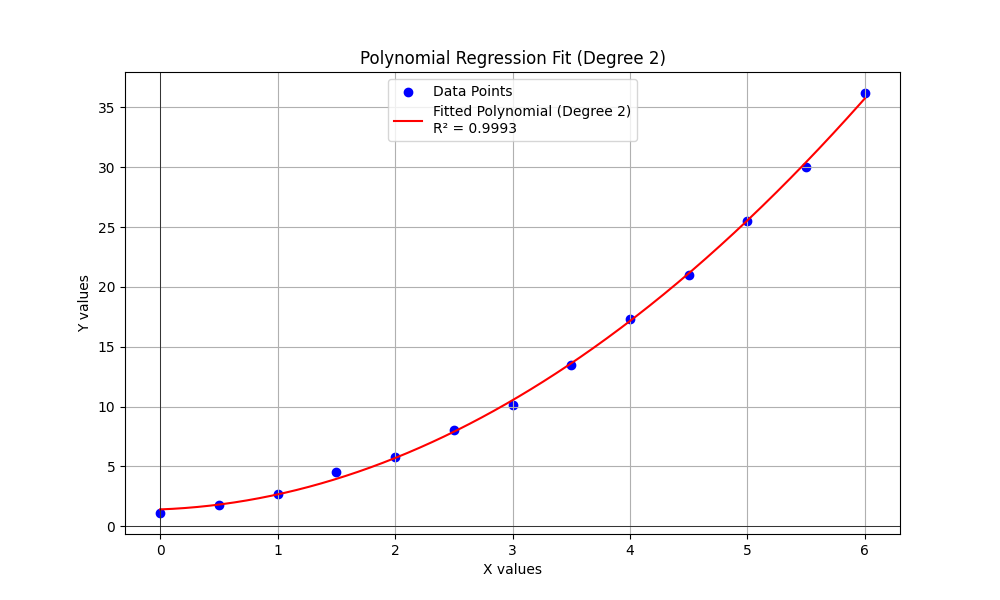
\includegraphics[width=0.9\columnwidth]{polynomial_regression_deg2.png}}
\caption{Hasil Regresi Polinomial (Derajat 2) pada Data Sintetis.}
\label{fig:poly_plot_deg2}
\end{figure}

Gambar \ref{fig:poly_plot_deg2} menunjukkan hasil visualisasi untuk regresi polinomial derajat 2 pada data sampel. Titik-titik biru merepresentasikan data asli dari \texttt{data.txt}, sedangkan garis merah adalah kurva polinomial derajat 2 yang dihitung oleh program C++. Nilai R-squared juga ditampilkan untuk menunjukkan kualitas kecocokan.

\begin{figure}[htbp]
\centerline{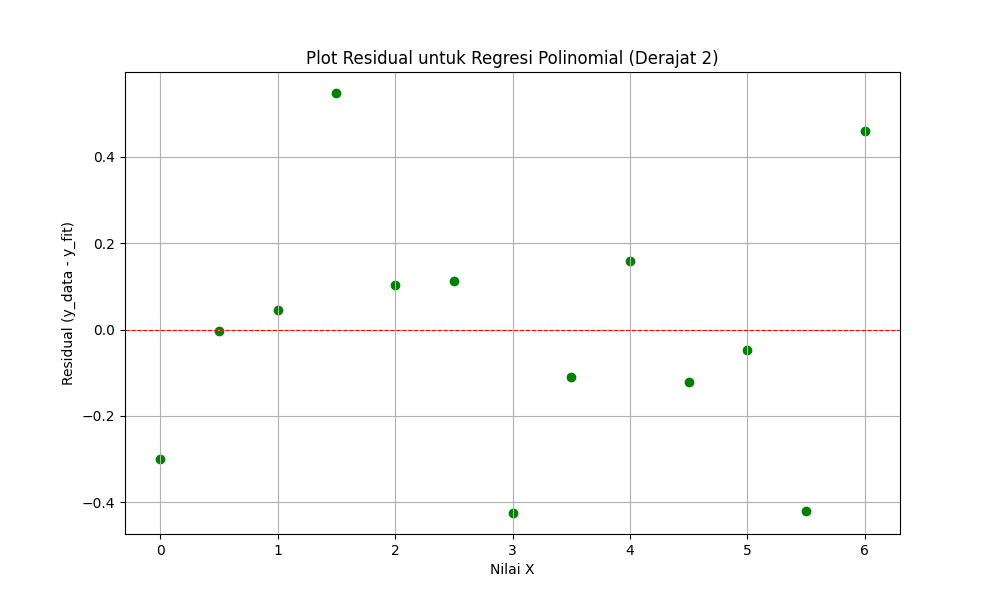
\includegraphics[width=0.9\columnwidth]{polynomial_regression_residuals_deg2.png}}
\caption{Plot Residual untuk Regresi Polinomial Derajat 2.}
\label{fig:residuals_deg2}
\end{figure}

Gambar \ref{fig:residuals_deg2} menampilkan plot residual untuk model regresi polinomial derajat 2. Residual adalah selisih antara nilai y aktual dan nilai y yang diprediksi oleh model. Idealnya, residual harus tersebar secara acak di sekitar garis nol. Hal ini menunjukkan bahwa model telah menangkap tren utama dalam data dan tidak ada pola sistematis yang tersisa.

\begin{figure}[htbp]
\centerline{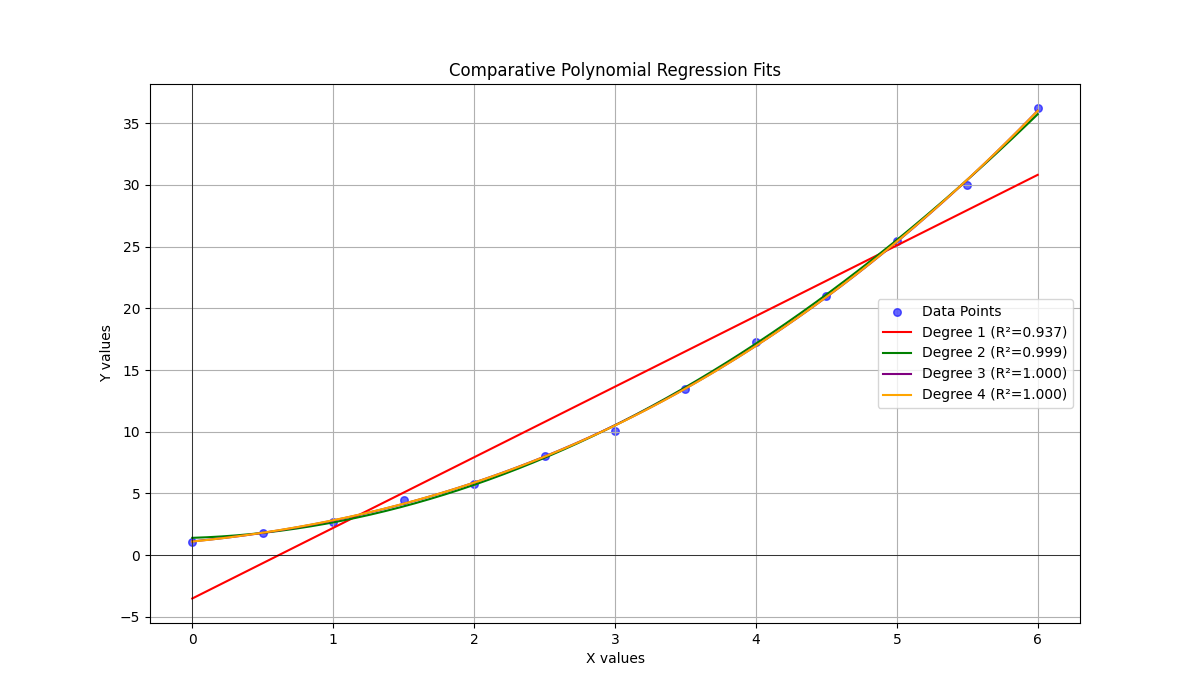
\includegraphics[width=0.9\columnwidth]{polynomial_regression_comparative_deg1_2_3_4.png}}
\caption{Perbandingan Hasil Regresi Polinomial untuk Derajat 1, 2, 3, dan 4.}
\label{fig:comparative_plot}
\end{figure}

Gambar \ref{fig:comparative_plot} menyajikan perbandingan kurva regresi untuk derajat polinomial 1, 2, 3, dan 4. Plot ini memungkinkan evaluasi visual tentang bagaimana peningkatan derajat polinomial memengaruhi kecocokan kurva terhadap data. Setiap kurva juga dilengkapi dengan nilai R-squared masing-masing.

\textbf{Analisis Hasil}:
\begin{itemize}
    \item \textbf{Kecocokan Kurva}: Dari Gambar \ref{fig:poly_plot_deg2} dan Gambar \ref{fig:comparative_plot}, dapat diamati bahwa kurva polinomial mampu mengikuti tren umum dari titik-titik data. Model regresi polinomial derajat 2 (parabola) tampak memberikan keseimbangan yang baik antara kecocokan dan kompleksitas untuk data sampel ini.
    \item \textbf{Plot Residual}: Plot residual pada Gambar \ref{fig:residuals_deg2} untuk derajat 2 menunjukkan bahwa titik-titik residual tersebar relatif acak di sekitar garis horizontal nol. Meskipun demikian, mungkin ada sedikit pola kurva yang tersisa. Ini bisa mengindikasikan bahwa model derajat 2 mungkin belum sepenuhnya menangkap semua struktur dalam data, atau bisa juga karena sifat dari noise yang ada pada data.
    \item \textbf{Pengaruh Derajat Polinomial}: Gambar \ref{fig:comparative_plot} secara jelas menunjukkan efek dari perubahan derajat:
    \begin{itemize}
        \item Derajat 1 (regresi linear) menghasilkan garis lurus. Ini jelas merupakan underfitting untuk data yang melengkung, yang juga ditunjukkan dengan nilai R-squared yang lebih rendah.
        \item Derajat 2 dan 3 memberikan kecocokan yang lebih baik. Nilai R-squared meningkat dari derajat 1 ke 2, dan sedikit lagi ke derajat 3.
        \item Model derajat 4 memberikan kecocokan yang sangat serupa dengan model derajat 3 untuk data ini. Nilai R-squared mungkin hanya sedikit lebih tinggi, atau bahkan identik. Menaikkan kompleksitas model dari derajat 3 ke 4 bisa jadi tidak menghasilkan perbaikan yang berarti untuk set data ini. Justru, hal ini dapat meningkatkan risiko \textit{overfitting}, terutama jika data mengandung lebih banyak \textit{noise} atau jika jumlah titik data relatif sedikit.
    \end{itemize}
    \item \textbf{Akurasi Metode Numerik}: Akurasi koefisien yang dihitung dipengaruhi oleh stabilitas numerik metode eliminasi Gauss. Selain itu, kondisi matriks normal equations ($\mathbf{X}^T\mathbf{X}$) juga berperan. Matriks ini dapat menjadi \textit{ill-conditioned} jika derajat polinomial sangat tinggi atau rentang data $x$ sangat besar. Matriks yang \textit{ill-conditioned} dapat menghasilkan solusi yang kurang akurat. Penggunaan presisi ganda (\texttt{double}) dalam C++ membantu memitigasi masalah ini.
    \item \textbf{Output Program}: Program C++ juga mencetak matriks normal equations dan vektor sisi kanan, serta koefisien yang dihitung ke konsol. Output ini berguna untuk debugging dan verifikasi selama proses pengembangan.
\end{itemize}

Secara keseluruhan, eksperimen menunjukkan bahwa implementasi regresi polinomial berfungsi sesuai harapan. Kombinasi C++ untuk komputasi numerik inti dan Python untuk visualisasi menyediakan alur kerja yang efektif untuk analisis data semacam ini.

\section{Kesimpulan}
Proyek ini berhasil mengimplementasikan metode regresi polinomial untuk analisis data eksperimental. Program inti dikembangkan dalam C++ untuk menghitung koefisien polinomial menggunakan metode normal equations yang diselesaikan dengan eliminasi Gauss. Data input dibaca dari file teks, dan koefisien yang dihasilkan disimpan ke file lain. Untuk visualisasi, skrip Python digunakan untuk memplot data asli bersama dengan kurva regresi polinomial yang telah dihitung, memberikan evaluasi visual terhadap kecocokan model.

Dari hasil eksperimen menggunakan data sintetis, dapat disimpulkan bahwa:
\begin{enumerate}
    \item Implementasi regresi polinomial mampu menangkap tren non-linear dalam data secara efektif, sebagaimana ditunjukkan oleh plot yang dihasilkan.
    \item Pemilihan derajat polinomial adalah faktor kunci yang memengaruhi kualitas kecocokan model. Plot perbandingan dan nilai R-squared membantu dalam memilih derajat yang sesuai untuk menghindari underfitting dan overfitting. Untuk data yang digunakan, derajat 2 atau 3 tampaknya memberikan hasil yang baik.
    \item Kombinasi C++ untuk komputasi numerik dan Python untuk visualisasi merupakan pendekatan yang kuat dan fleksibel untuk tugas-tugas analisis data numerik.
    \item Metode numerik yang digunakan, seperti eliminasi Gauss, terbukti cukup untuk menyelesaikan sistem persamaan linear yang muncul dalam konteks regresi ini untuk data dan derajat polinomial yang wajar.
\end{enumerate}
Proyek ini memberikan pemahaman praktis tentang penerapan salah satu metode pencocokan kurva yang fundamental dalam komputasi numerik dan analisis data.

\section*{Link Github}
Repositori Github untuk proyek ini dapat diakses melalui link berikut:
\href{https://github.com/IfanFYS/Proyek-UAS-Komnum}{\textit{\underline{https://github.com/IfanFYS/Proyek-UAS-Komnum}}}

\section*{Link Youtube}
Video demonstrasi program dapat dilihat di Youtube melalui link berikut:
% Ganti placeholder di bawah ini dengan link YouTube Anda menggunakan format:
% \href{URL_YOUTUBE_ANDA}{\textit{\underline{URL_YOUTUBE_ANDA}}}
% Contoh (jika URL mengandung underscore, escape pada bagian teks): 
% \href{https://www.youtube.com/watch?v=a_b-c_d}{\textit{\underline{https://www.youtube.com/watch?v=a\_b-c\_d}}}
\href{https://youtu.be/icb7CtffLWc}{\textit{\underline{https://youtu.be/icb7CtffLWc}}}

\section*{Referensi}
% Please number citations consecutively within brackets \cite{b1}. 
% The sentence punctuation follows the bracket \cite{b2}. Refer simply to the reference 
% number, as in \cite{b3}---do not use ``Ref. \cite{b3}'' or ``reference \cite{b3}'' except at 
% the beginning of a sentence: ``Reference \cite{b3} was the first $\ldots$''

% Number footnotes separately in superscripts. Place the actual footnote at 
% the bottom of the column in which it was cited. Do not put footnotes in the 
% abstract or reference list. Use letters for table footnotes.

% Unless there are six authors or more give all authors' names; do not use 
% ``et al.''. Papers that have not been published, even if they have been 
% submitted for publication, should be cited as ``unpublished'' \cite{b4}. Papers 
% that have been accepted for publication should be cited as ``in press'' \cite{b5}. 
% Capitalize only the first word in a paper title, except for proper nouns and 
% element symbols.

% For papers published in translation journals, please give the English 
% citation first, followed by the original foreign-language citation \cite{b6}.

\begin{thebibliography}{00}
\bibitem{b1} Chapra, S. C., & Canale, R. P. (2015). \textit{Numerical Methods for Engineers} (7th ed.). McGraw-Hill Education. (Terutama Bab 17 untuk Regresi Polinomial dan Bab 9-10 untuk Eliminasi Gauss).
\bibitem{b2} James, G., Witten, D., Hastie, T., & Tibshirani, R. (2013). \textit{An Introduction to Statistical Learning: with Applications in R}. Springer. (Bab 7 membahas model regresi non-linear termasuk regresi polinomial).
\bibitem{b3} Press, W. H., Teukolsky, S. A., Vetterling, W. T., & Flannery, B. P. (2007). \textit{Numerical Recipes: The Art of Scientific Computing} (3rd ed.). Cambridge University Press.
% \bibitem{b4} K. Elissa, ``Title of paper if known,'' unpublished.
% \bibitem{b5} R. Nicole, ``Title of paper with only first word capitalized,'' J. Name Stand. Abbrev., in press.
% \bibitem{b6} Y. Yorozu, M. Hirano, K. Oka, and Y. Tagawa, ``Electron spectroscopy studies on magneto-optical media and plastic substrate interface,'' IEEE Transl. J. Magn. Japan, vol. 2, pp. 740--741, August 1987 [Digests 9th Annual Conf. Magnetics Japan, p. 301, 1982].
% \bibitem{b7} M. Young, The Technical Writer's Handbook. Mill Valley, CA: University Science, 1989.
\end{thebibliography}
\vspace{12pt}
% \color{red}
% IEEE conference templates contain guidance text for composing and formatting conference papers. Please ensure that all template text is removed from your conference paper prior to submission to the conference. Failure to remove the template text from your paper may result in your paper not being published.

\end{document}
